
\documentclass[journal]{IEEEtran}

\usepackage{epsfig,graphicx,lineno,amssymb,mdwmath,array,amsmath}
\usepackage{subfigure}
\usepackage{multirow}
\usepackage{xcolor}
\usepackage{cite}
\usepackage{epstopdf}
\newtheorem{mydef}{Definition}
\newtheorem{mylem}{Lemma}
\newtheorem{mythm}{Theorem}
\newtheorem{cor}{Corollary}

\hyphenation{op-tical net-works semi-conduc-tor}


\begin{document}
%
% paper title
% can use linebreaks \\ within to get better formatting as desired
% Do not put math or special symbols in the title.
\title{An Rssi-Based Wifi Access Management Approach for Energy Saving on Smartphones}
%
%
% author names and IEEE memberships
% note positions of commas and nonbreaking spaces ( ~ ) LaTeX will not break
% a structure at a ~ so this keeps an author's name from being broken across
% two lines.
% use \thanks{} to gain access to the first footnote area
% a separate \thanks must be used for each paragraph as LaTeX2e's \thanks
% was not built to handle multiple paragraphs
%

\author{Lunde~Chen,
        ~Huan~Li*,~\IEEEmembership{Member,~IEEE,}% <-this % stops a space
\thanks{*Corresponding Author: H. Li,  is with the School
of Computer Science and Engineering, Beihang University, Beijing,
China 100191,  e-mail: (lihuan@buaa.edu.cn.}% <-this % stops a space
\thanks{L. Chen is with with the School of Computer Science and Engineering and Ecole Centrale de Pékin, Beihang University, Beijing, China 100191.}% <-this % stops a space
\thanks{Manuscript received September 15, 2014.}}

% note the % following the last \IEEEmembership and also \thanks - 
% these prevent an unwanted space from occurring between the last author name
% and the end of the author line. i.e., if you had this:
% 
% \author{....lastname \thanks{...} \thanks{...} }
%                     ^------------^------------^----Do not want these spaces!
%
% a space would be appended to the last name and could cause every name on that
% line to be shifted left slightly. This is one of those "LaTeX things". For
% instance, "\textbf{A} \textbf{B}" will typeset as "A B" not "AB". To get
% "AB" then you have to do: "\textbf{A}\textbf{B}"
% \thanks is no different in this regard, so shield the last } of each \thanks
% that ends a line with a % and do not let a space in before the next \thanks.
% Spaces after \IEEEmembership other than the last one are OK (and needed) as
% you are supposed to have spaces between the names. For what it is worth,
% this is a minor point as most people would not even notice if the said evil
% space somehow managed to creep in.



% The paper headers
\markboth{IEEE EMBEDDED SYSTEMS LETTERS}%%Journal of \LaTeX\ Class Files,~Vol.~11, No.~4, December~2012}%
{Shell \MakeLowercase{\textit{et al.}}: Bare Demo of IEEEtran.cls for Journals}
% The only time the second header will appear is for the odd numbered pages
% after the title page when using the twoside option.
% 
% *** Note that you probably will NOT want to include the author's ***
% *** name in the headers of peer review papers.                   ***
% You can use \ifCLASSOPTIONpeerreview for conditional compilation here if
% you desire.




% If you want to put a publisher's ID mark on the page you can do it like
% this:
%\IEEEpubid{0000--0000/00\$00.00~\copyright~2012 IEEE}
% Remember, if you use this you must call \IEEEpubidadjcol in the second
% column for its text to clear the IEEEpubid mark.



% use for special paper notices
%\IEEEspecialpapernotice{(Invited Paper)}




% make the title area
\maketitle

% As a general rule, do not put math, special symbols or citations
% in the abstract or keywords.
\begin{abstract}
The abstract goes here.
\end{abstract}

% Note that keywords are not normally used for peerreview papers.
\begin{IEEEkeywords}
Rssi, Energy saving, algorithm.
\end{IEEEkeywords}



% For peer review papers, you can put extra information on the cover
% page as needed:
% \ifCLASSOPTIONpeerreview
% \begin{center} \bfseries EDICS Category: 3-BBND \end{center}
% \fi
%
% For peerreview papers, this IEEEtran command inserts a page break and
% creates the second title. It will be ignored for other modes.
\IEEEpeerreviewmaketitle



\section{Introduction}
% The very first letter is a 2 line initial drop letter followed
% by the rest of the first word in caps.
% 
% form to use if the first word consists of a single letter:
% \IEEEPARstart{A}{demo} file is ....
% 
% form to use if you need the single drop letter followed by
% normal text (unknown if ever used by IEEE):
% \IEEEPARstart{A}{}demo file is ....
% 
% Some journals put the first two words in caps:
% \IEEEPARstart{T}{his demo} file is ....
% 
% Here we have the typical use of a "T" for an initial drop letter
% and "HIS" in caps to complete the first word.
\IEEEPARstart{G}{uidance}: This paragraph is to address 1) the growth of the multimedia applications on smartphone [Need some data evidence], and most need download large files, e.g., app tar files and movies etc. 2) the wifi access requirements for those applications, and 3) major Wifi properties and the impact on the critical energy issues on resource-constrained smartphones. 

{[\bf Guidance:]}  1) The most widely used energy-efficient wifi access strategies, such as prediction sleeping methods are introduced here,  2) The limits or problems of those strategies.

{[\bf Guidance:]} The contributions of this paper: 1) extensive experiments to evaluate the relationship of rssi and the energy consumption, 2) propose a novel Rssi-based wifi access management algorithm, 3) effectiveness evaluation using simulations.
% You must have at least 2 lines in the paragraph with the drop letter
% (should never be an issue)


%\hfill mds
 
%\hfill December 27, 2012  

\section{Evaluation of Rssi and Energy Consumption}
\subsection{Settings and Methodology}
{[\bf Guidance:]} Experimental environment and settings

\subsection{Experimental Setup for Rssi Charactirization}

\subsection{Experimental Setup for Power Measurement}
This section describes the experimental setup for power measurement. The Android smartphone used 
is a Huawei 8950D with superuser access. Its hardware specifications are shown is Table 1. 
The smartphone is equiped with Iptables and Tcpdump that are cross compiled. 
(Or to say:We cross compile Iptables and Tcpdump and install them into the smartphone as local libararies).
Iptables is used to block the Internet access of unrelated applications to avoid GANRAO traffic. 
Tcpdump is used to analyse traffic information when downloading files at different Rssi. 
\\  
\indent  We use a Monsoon Power Monitor for power measurement. The measurement instruments are illustrated in Figure 1.
The Monsoon Power Monitor supplies a stable voltage of 3.7V to the smartphone and samples the power consumption at a rate of 5KHz. 
\\  
\indent  We adjust the distance between the smartphone and the AP to get different Rssi. 
When we perform measurements, we keep all instruments at fixed location. 
We develop an application (WiDownload) that download files 
using the DownloadManager API provided by Android. We use Iptables to block the Internet access of all applications 
except that of WiDownload so that no GANRAO traffic is introduced. 
During the download, the screen is off and the WifiLock is aquired. 
\\  
\indent We measure the power consumed for 
completing downloading a file of 11.4 Mb. After this, we perform a same download at the same fixed location, but with 
Tcpdump running to dump traffic information. Each measurement is repeated 3 times. After that, we move the instruments to 
another location where the Rssi is different and reconduct the experiment. 

{[\bf Guidance:]} We measure....

\subsection{Results}
Put the figures and analysis here.
\\
\indent Figure 1 shows the power consumption for the download at strong (-30 dBm) and relatively weak (-80 dBm) Rssi.

% if error, type "pdflatex --shell-escape Version-1.tex" in Terminal
\begin{figure}
\centering
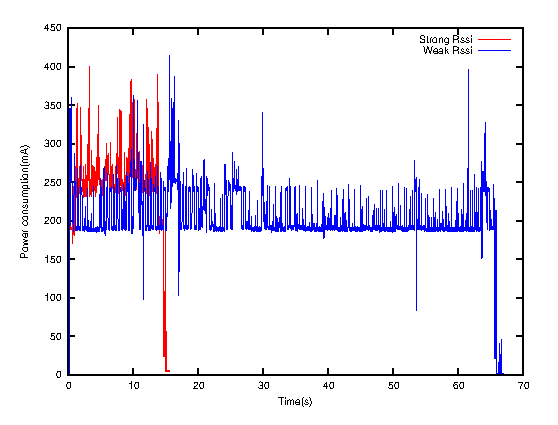
\includegraphics[scale=1]{energy_comparision.eps}
\caption{Power consumption for downloading a file (11.4Mb) in different Rssi}
\end{figure}

Figure 3 and 4 are the corresponding traffic throughput.

\begin{figure}
\centering
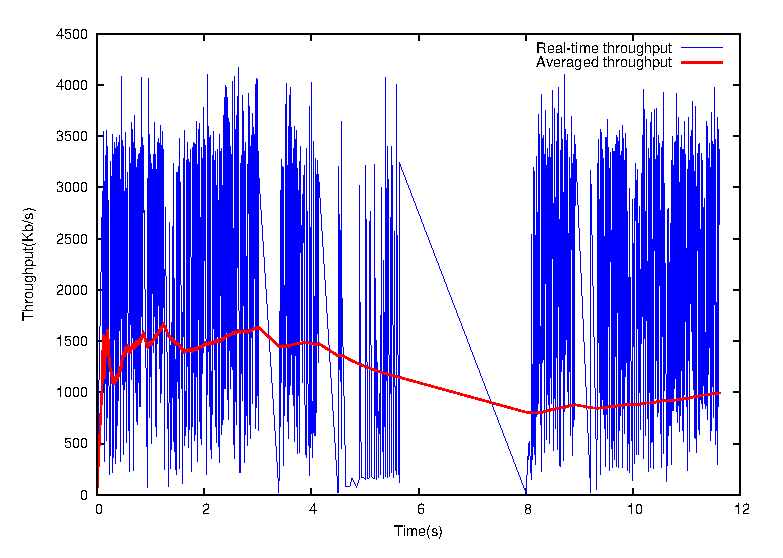
\includegraphics[scale=0.55]{strong_traffic.eps}
\caption{Throughput in strong Rssi}
\end{figure}

\begin{figure}
\centering
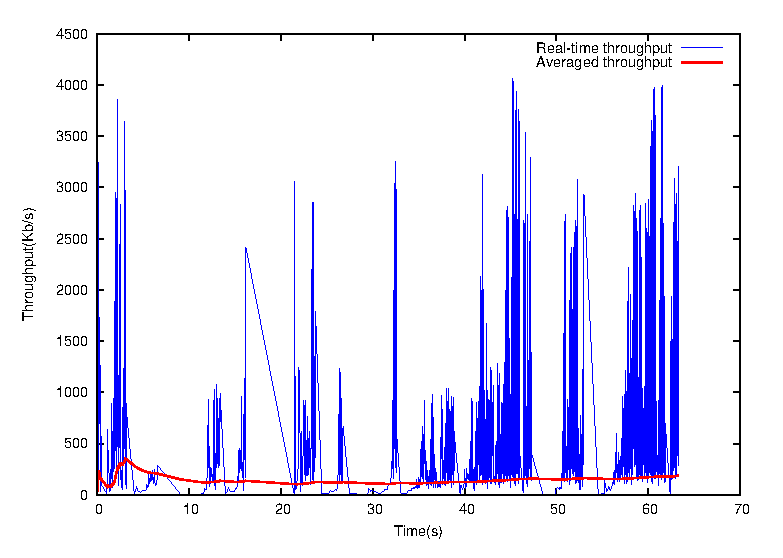
\includegraphics[scale=0.55]{weak_traffic.eps}
\caption{Throughput in weak Rssi}
\end{figure}

\indent The whole dataset is plotted in Figure 5. We 

\begin{figure}
\centering
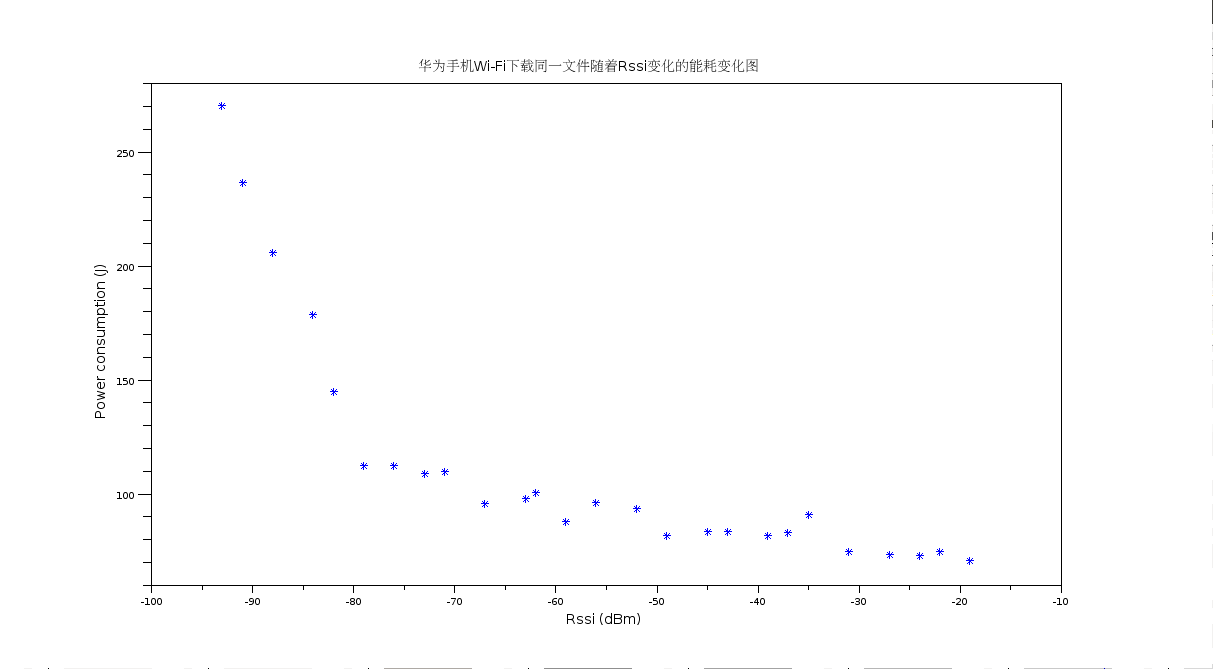
\includegraphics[scale=0.2]{energy_different_rssi.png}
\caption{Energy Consumption is different Rssi}
\end{figure}

\indent We conclude that when the Rssi is weak, the energy consumption for downloading files increases drammatically. 
One straight-forward propostion for energy saving is to close the Wi-Fi interface when Rssi is weak and re-opening is when Rssi 
is strong. To invastigate the possiblity of this solution, 
we measure the energy consumption for opening and close the Wi-Fi interface. The measurement result is shown in Figure 6.
\\
\indent 


\section{Rssi-based Wifi Access Algorithm}

Algorithm statement and pseudo-code

\section{Simulation Results}
{[\bf Guidance:]} Simulation Methodology

{[\bf Guidance:]} Comparison results

% An example of a floating figure using the graphicx package.
% Note that \label must occur AFTER (or within) \caption.
% For figures, \caption should occur after the \includegraphics.
% Note that IEEEtran v1.7 and later has special internal code that
% is designed to preserve the operation of \label within \caption
% even when the captionsoff option is in effect. However, because
% of issues like this, it may be the safest practice to put all your
% \label just after \caption rather than within \caption{}.
%
% Reminder: the "draftcls" or "draftclsnofoot", not "draft", class
% option should be used if it is desired that the figures are to be
% displayed while in draft mode.
%
%\begin{figure}[!t]
%\centering
%\includegraphics[width=2.5in]{myfigure}
% where an .eps filename suffix will be assumed under latex, 
% and a .pdf suffix will be assumed for pdflatex; or what has been declared
% via \DeclareGraphicsExtensions.
%\caption{Simulation Results.}
%\label{fig_sim}
%\end{figure}

% Note that IEEE typically puts floats only at the top, even when this
% results in a large percentage of a column being occupied by floats.


% An example of a double column floating figure using two subfigures.
% (The subfig.sty package must be loaded for this to work.)
% The subfigure \label commands are set within each subfloat command,
% and the \label for the overall figure must come after \caption.
% \hfil is used as a separator to get equal spacing.
% Watch out that the combined width of all the subfigures on a 
% line do not exceed the text width or a line break will occur.
%
%\begin{figure*}[!t]
%\centering
%\subfloat[Case I]{\includegraphics[width=2.5in]{box}%
%\label{fig_first_case}}
%\hfil
%\subfloat[Case II]{\includegraphics[width=2.5in]{box}%
%\label{fig_second_case}}
%\caption{Simulation results.}
%\label{fig_sim}
%\end{figure*}
%
% Note that often IEEE papers with subfigures do not employ subfigure
% captions (using the optional argument to \subfloat[]), but instead will
% reference/describe all of them (a), (b), etc., within the main caption.


% An example of a floating table. Note that, for IEEE style tables, the 
% \caption command should come BEFORE the table. Table text will default to
% \footnotesize as IEEE normally uses this smaller font for tables.
% The \label must come after \caption as always.
%
%\begin{table}[!t]
%% increase table row spacing, adjust to taste
%\renewcommand{\arraystretch}{1.3}
% if using array.sty, it might be a good idea to tweak the value of
% \extrarowheight as needed to properly center the text within the cells
%\caption{An Example of a Table}
%\label{table_example}
%\centering
%% Some packages, such as MDW tools, offer better commands for making tables
%% than the plain LaTeX2e tabular which is used here.
%\begin{tabular}{|c||c|}
%\hline
%One & Two\\
%\hline
%Three & Four\\
%\hline
%\end{tabular}
%\end{table}


% Note that IEEE does not put floats in the very first column - or typically
% anywhere on the first page for that matter. Also, in-text middle ("here")
% positioning is not used. Most IEEE journals use top floats exclusively.
% Note that, LaTeX2e, unlike IEEE journals, places footnotes above bottom
% floats. This can be corrected via the \fnbelowfloat command of the
% stfloats package.



\section{Conclusion}
The conclusion goes here.





% if have a single appendix:
%\appendix[Proof of the Zonklar Equations]
% or
%\appendix  % for no appendix heading
% do not use \section anymore after \appendix, only \section*
% is possibly needed

% use appendices with more than one appendix
% then use \section to start each appendix
% you must declare a \section before using any
% \subsection or using \label (\appendices by itself
% starts a section numbered zero.)
%

\iffalse
\appendices
\section{Proof of the First Zonklar Equation}
Appendix one text goes here.

% you can choose not to have a title for an appendix
% if you want by leaving the argument blank
\section{}
Appendix two text goes here.

\fi

% use section* for acknowledgement
\section*{Acknowledgment}

This work is supported by the National Nature Science Foundation of China, NSFC (Grant No. 61170293) and the International Science \& Technology Cooperation Program of China, Ministry of Science and Technology of China (Grant No. 2014DFG12370).

% Can use something like this to put references on a page
% by themselves when using endfloat and the captionsoff option.
\ifCLASSOPTIONcaptionsoff
  \newpage
\fi



% trigger a \newpage just before the given reference
% number - used to balance the columns on the last page
% adjust value as needed - may need to be readjusted if
% the document is modified later
%\IEEEtriggeratref{8}
% The "triggered" command can be changed if desired:
%\IEEEtriggercmd{\enlargethispage{-5in}}

% references section

% can use a bibliography generated by BibTeX as a .bbl file
% BibTeX documentation can be easily obtained at:
% http://www.ctan.org/tex-archive/biblio/bibtex/contrib/doc/
% The IEEEtran BibTeX style support page is at:
% http://www.michaelshell.org/tex/ieeetran/bibtex/
%\bibliographystyle{IEEEtran}
% argument is your BibTeX string definitions and bibliography database(s)
%\bibliography{IEEEabrv,../bib/paper}
%
% <OR> manually copy in the resultant .bbl file
% set second argument of \begin to the number of references
% (used to reserve space for the reference number labels box)
\begin{thebibliography}{1}

\bibitem{IEEEhowto:kopka}
H.~Kopka and P.~W. Daly, \emph{A Guide to \LaTeX}, 3rd~ed.\hskip 1em plus
  0.5em minus 0.4em\relax Harlow, England: Addison-Wesley, 1999.

\end{thebibliography}

% biography section
% 
% If you have an EPS/PDF photo (graphicx package needed) extra braces are
% needed around the contents of the optional argument to biography to prevent
% the LaTeX parser from getting confused when it sees the complicated
% \includegraphics command within an optional argument. (You could create
% your own custom macro containing the \includegraphics command to make things
% simpler here.)
%\begin{IEEEbiography}[{\includegraphics[width=1in,height=1.25in,clip,keepaspectratio]{mshell}}]{Michael Shell}
% or if you just want to reserve a space for a photo:

\iffalse
\begin{IEEEbiography}{Michael Shell}
Biography text here.
\end{IEEEbiography}

% if you will not have a photo at all:
\begin{IEEEbiographynophoto}{John Doe}
Biography text here.
\end{IEEEbiographynophoto}

% insert where needed to balance the two columns on the last page with
% biographies
%\newpage

\begin{IEEEbiographynophoto}{Jane Doe}
Biography text here.
\end{IEEEbiographynophoto}

\fi

% You can push biographies down or up by placing
% a \vfill before or after them. The appropriate
% use of \vfill depends on what kind of text is
% on the last page and whether or not the columns
% are being equalized.

%\vfill

% Can be used to pull up biographies so that the bottom of the last one
% is flush with the other column.
%\enlargethispage{-5in}



% that's all folks
\end{document}


